\documentclass[fleqn,10pt]{wlscirep}
\usepackage[utf8]{inputenc}
\usepackage[T1]{fontenc}
\usepackage{textcomp}
\usepackage{graphicx}
\usepackage{tablefootnote}
\usepackage{xr}

\makeatletter
\newcommand*{\addFileDependency}[1]{% argument=file name and extension
  \typeout{(#1)}
  \@addtofilelist{#1}
  \IfFileExists{#1}{}{\typeout{No file #1.}}
}
\makeatother

\newcommand{\iu}{{i\mkern1mu}}

\newcommand*{\myexternaldocument}[1]{%
    \externaldocument{#1}%
    \addFileDependency{#1.tex}%
    \addFileDependency{#1.aux}%
}

\myexternaldocument{SI}

\title{NMRlipids Databank makes data-driven analysis of biomembrane properties accessible for all}
%NMRlipids Databank: Making data-driven analyses of membrane properties accessible for all^
%Overlay Databank of Lipid Membrane Simulations Arising from Open Collaboration

\author[1]{Anne M. Kiirikki}         %ORCID: ?
\author[2,3]{Hanne S. Antila}          %ORCID: 0000-0002-2474-5053
\author[2,4]{Lara S. Bort}             %ORCID: ?
\author[5]{Pavel Buslaev}         %ORCID: 0000-0003-2031-4691
\author[6]{Fernando Favela-Rosales}
\author[7]{Tiago Mendes Ferreira}
\author[8,9]{Patrick F.J. Fuchs}
\author[10]{Rebeca Garcia-Fandino}
\author[11]{Ivan Gushchin}
%\author[2]{Matti Javanainen}      %ORCID: 0000-0003-4858-364X
\author[12,13]{Batuhan Kav}           %ORCID: 0000-0003-4990-373X
\author[14]{Norbert Ku{\v c}erka}
\author[15]{Patrik Kula}
\author[16]{Milla Kurki}
\author[11]{Alexander Kuzmin}
\author[17,18]{Jesper J. Madsen}  %ORCID: 0000-0003-1411-9080
\author[2,19,20]{Markus S. Miettinen}   %ORCID: 0000-0002-3999-4722
%\author[2]{...}                   %ORCID: ?
\author[1]{Ricky Nencini}
\author[21]{Thomas J. Piggot}
\author[22]{{\'A}ngel Pi{\~n}eiro}
%\author[11]{Suman Samantray} %ORCID: 0000-0003-3361-9582
\author[10,22,23]{Fabi{\'a}n Su{\'a}rez-Lest{\'o}n}
\author[1,24,*]{O. H. Samuli Ollila} %ORCID: 0000-0002- 8728-1006
%\author[1,2,+]{Christine Author}
%\author[2,+]{Derek Author}

\affil[1]{University of Helsinki, Institute of Biotechnology, Helsinki, Finland}
\affil[2]{Department of Theory and Bio-Systems, Max Planck Institute of Colloids and Interfaces, 14424 Potsdam, Germany}
\affil[3]{Department of Biomaterials, Max Planck Institute of Colloids and Interfaces, 14424 Potsdam, Germany}
\affil[4]{University of Potsdam, Institute of Physics and Astronomy, Potsdam-Golm, 14476, Germany}
%\affil[2]{Affiliation, department, city, postcode, country}
\affil[5]{Nanoscience Center and Department of Chemistry, University of Jyv{\"a}skyl{\"a}, P.O. Box 35, Jyv{\"a}skyl{\"a}, 40014 , Finland}
\affil[6]{Departamento de Ciencias B\'{a}sicas, Tecnol\'{o}gico Nacional de M\'{e}xico - ITS Zacatecas Occidente, Sombrerete, Zacatecas, 99102, M\'{e}xico}
\affil[7]{NMR group - Institute for Physics, Martin Luther University Halle-Wittenberg,  Halle (Saale), 06120, Germany}
\affil[8]{Sorbonne Universit{\'e}, Ecole Normale Sup{\'e}rieure, PSL University, CNRS, Laboratoire des Biomol{\'e}cules (LBM), Paris, 75005, France}
\affil[9]{Universit{\'e} Paris Cit{\'e}, UFR Sciences du Vivant, Paris, 75013, France}
\affil[10]{Center for Research in Biological Chemistry and Molecular Materials (CiQUS), Universidade de Santiago de Compostela,  Santiago de Compostela, E-15782, Spain}
\affil[11]{no affiliation}
%Physical and Computational Sciences Division, Pacific Northwest National Laboratory, Richland, Washington 99352, United States
\affil[12]{Institute of Biological Information Processing: Structural Biochemistry (IBI-7), Forschungszentrum Jülich, Jülich 52428, Germany}
\affil[13]{ariadne.ai GmbH (Germany), Häusserstra{\ss}e 3 Heidelberg 69115, Germany }
\affil[14]{Department of Physical Chemistry of Drugs and Faculty of Pharmacy, Comenius University Bratislava, 832 32 Bratislava, Slovakia}
\affil[15]{Institute of Organic Chemistry and Biochemistry of the Czech Academy of Sciences, Flemingovo n\'{a}m. 542/2,  Prague, CZ-16610, Czech Republic}
\affil[16]{School of Pharmacy, University of Eastern Finland, 70211 Kuopio, Finland}
\affil[17]{Global and Planetary Health, College of Public Health, University of South Florida, Tampa, Florida, 33612, United States of America}
\affil[18]{Department of Molecular Medicine, Morsani College of Medicine, University of South Florida, Tampa, Florida, 33612, United States of America}
\affil[19]{Department of Chemistry, University of Bergen, 5020 Bergen, Norway}
\affil[20]{Computational Biology Unit, Department of Informatics, University of Bergen, 5020 Bergen, Norway}
\affil[21]{Chemistry, University of Southampton, Highfield, Southampton, SO17 1BJ, United Kingdom}
\affil[22]{Department of Applied Physics, Faculty of Physics, University of Santiago de Compostela, Santiago de Compostela, E-15782, Spain}
\affil[23]{MD.USE Innovations S.L., Edificio Emprendia, 15782 Santiago de Compostela, Spain}
\affil[24]{VTT Technical Research Centre of Finland, Espoo, Finland}

\affil[*]{samuli.ollila@helsinki.fi}

%\affil[+]{these authors contributed equally to this work}

%\keywords{Keyword1, Keyword2, Keyword3}

\begin{abstract}
Cellular membrane lipid composition is implicated in diseases and controls major biological functions, but membranes are difficult to study experimentally due to their intrinsic disorder and complex phase behaviour. Molecular dynamics (MD) simulations have been useful in understanding membrane systems, but they require significant computational resources and often suffer from inaccuracies in model parameters. Applications of data-driven and machine learning methods, currently revolutionising many fields, remain of limited use for membrane systems due to the lack of suitable training sets. Here we present the NMRlipids Databank---a community-driven, open-for-all database featuring programmatic access to quality-evaluated atom-resolution MD simulations of lipid bilayers. The NMRlipids Databank will benefit scientists in different disciplines by providing automatic ranking of simulations based on their quality against experiments, programmable interface for flexible implementation of data-driven and machine learning applications, and rapid access to simulation data through a graphical user interface. To demonstrate how it unlocks possibilities beyond current MD simulation studies, we analyzed the NMRlipids Databank to reveal how anisotropic diffusion of water and cholesterol flip-flop rates depend on membrane properties.

\end{abstract}
\begin{document}

\flushbottom
\maketitle
% * <john.hammersley@gmail.com> 2015-02-09T12:07:31.197Z:
%
%  Click the title above to edit the author information and abstract
%
\thispagestyle{empty}

%\noindent Please note: Abbreviations should be introduced at the first mention in the main text – no abbreviations lists. Suggested structure of main text (not enforced) is provided below.

\section{Introduction}

%The demand for sharing and reusing of MD simulation data is increasing, but practical solution remains unclear due to unsolved issues in data storage and indexing.

Cellular membranes contain hundreds of different types of lipid molecules that regulate the membrane properties, morphology, and biological functions~\cite{vanmeer08,Lorent:2020a,Slatter:2016a}. Membrane lipid composition is implicated in diseases, such as cancer and neurodegenerative disorders, and therapeutics that affect membrane compositions are emerging~\cite{torres21}. However, biomembranes are often difficult to study experimentally, because they are complex mixtures of proteins and lipids in disordered fluid state with complicated phase behaviour at physiologicalbiological conditions. For those reasons, the detailed connections between complex lipid interactions and biological functions taking place in or around membranes remain poorly understood. Molecular dynamics (MD) simulations have been particularly useful in understanding membrane systems, although their accuracy has often been compromised by artefacts such as the quality of model parameters~\cite{antila22b,gupta22}. Presently, the accuracy of models is becoming increasingly important as researches are progressing from simulations of individual molecules to simulating whole organelles or even cells using interdisciplinary approaches~\cite{johnson15,thornburg22,gupta22}. Such systems exhibit intricate emergent behaviour making inaccuracies more difficult to detect, and accumulation of even modest errors may have a dramatic impact on the conclusions drawn.

In contrast to experimental structural biology, where standard protocols to share and quality-evaluate resolved biomolecular structures are firmly established by the Protein Data Bank (PDB)~\cite{montelione13}, equivalent best practices are yet to be defined for MD simulations. The importance of such approaches is widely recognized~\cite{feig99,tai04,silva06,abraham19,hildebrand19,hospital20,abriata20,espigares20} and data-sharing solutions are emerging for proteins in solution~\cite{meyer10,kamp10}, proteins in membranes~\cite{newport19,espigares20,leston22}, nucleic acids~\cite{hospital16}, nucleic acids and proteins~\cite{bekker20}, cyclodextrins~\cite{mixcoha16}, COVID-19--involved macromolecules~(\href{https://bioexcel-cv19.bsc.es}{bioexcel-cv19.bsc.es}). However, automatic quality evaluation of simulation data~\cite{meyer10,hospital16} and programmatic access are still rare. In particular, tools for automatic quality evaluation of membrane simulations, or training sets for machine learning models of membrane-containing systems, are not yet available. Recent advances using machine learning approaches utilizing publicly available databanks, for example to solve protein structures~\cite{jumper21}, emphasize the increasing importance of such resources. 

Here we present the NMRlipids Databank --- a community-driven, open-for-all database featuring programmatic access to atom-resolution MD simulations of lipid bilayers. The programmatic access enables users to apply their data-driven approaches on the Databank, thus facilitating the creation of new tools for (and by) researchers in a wide range of fields covering academia and industry, from cell membrane biology and lipid nanoparticle formulations to computational chemistry and machine learning. As two usage examples of what is already possible, we demonstrate here (i) how data-driven analysis of water anisotropic diffusion in all the membrane systems available in the Databank can extend the scope of MD simulations to magnetic resonance imaging (MRI) and pharmacokinetics, and (ii) how the Databank allows its users to analyse rare phenomena that are beyond the scope of standard MD simulation investigations. Wider adaptation of the NMRlipids Databank will open even more possibilities. Furthermore, the Databank performs automatic quality evaluation of membrane simulations, which facilitates the selection of best-performing models for each given application and accelerates the development of simulation parameters and methodology.  


While the NMRlipids Databank currently contains only lipid bilayer systems, its key elements that enable programmatic access to large-scale MD simulation data can be applied also for other molecules, such as disordered proteins or sugars. The powerful combination of an overlay databank structure and a community-wide open collaboration can be used to build databases that enable data-driven and machine learning applications also in other fields, where storage of raw data requires significant resources, best practices in the field are not yet defined, and incentives to share data do not exist---such as assignment of NMR spectra~\cite{klukowski22}. 



\section{Results}

\subsection{MD simulations of membranes composed of the biologically most abundant lipids}

NMRlipids Databank is a community-driven catalogue containing atomistic MD simulations of biologically relevant lipid membranes emerging from the NMRlipids open collaboration~\cite{botan15,ollila16,catte16,antila19,bacle21}. It has been designed to improve the Findability, Accessibility, Interoperability, and Reuse (FAIR)~\cite{wilkinson16} of MD simulation data, most importantly the output trajectories and necessary information to their reuse. The NMRlipids Databank is constructed using the NMRlipids project protocol, in which all the content is openly accessible throughout the project~\cite{botan15}. Currently, the NMRlipids Databank contains 726 simulation trajectories with the total length of approximately 0.4\,ms. Single-component lipid membranes and binary mixtures, depicted in Fig.~\ref{fig:overlay}F, are currently most abundant in the NMRlipids Databank, yet mixtures with up to five lipid types are available. The distribution of lipids among the available simulations, shown in Fig.~\ref{fig:overlay}B, roughly resembles the biological relative abundance of different lipid types, with phosphatidylcholine (PC) being the most common followed by cholesterol, phosphatidylethanolamine (PE), phosphatidylserine (PS), phosphatidylglycerol (PG), phosphatidylinositol (PI), and other lipids, depending on organism and organelle~\cite{vanmeer08}. Abbreviations and full names of all lipids present in the Databank are listed in Table~\ref{tab:abbreviations}. Force fields used in simulations cover all the essential parameter sets commonly used in lipid simulations, see Fig.~\ref{fig:overlay}C and Table~\ref{tab:ForceFields}, including also united atom and polarizable force fields. Therefore, the averages calculated over the Databank can be considered as mean predictions from available lipid models (average over force field parameters) for an average cell membrane (average over lipid compositions).

The overlay structure of the NMRlipids Databank, illustrated in Fig.~\ref{fig:overlay}A, is designed to enable efficient upcycling of MD simulations for data-driven and machine learning applications with minimal investment on new infrastructure. Raw simulation data in the {\it Data layer} can be stored in any publicly available location with long term stability
%figshare (\href{https://figshare.com}{figshare.com}), or NIRD research data archive (\href{https://archive.norstore.no}{archive.norstore.no})---
and with permanent links to the data, such as digital object identifiers (DOIs), such as Zenodo (\href{https://zenodo.org}{zenodo.org}). 
%or uniform resource names (URNs). 
The {\it Databank layer} (\href{https://github.com/NMRlipids/Databank}{github.com/NMRlipids/Databank}) is the core of the Databank containing all the relevant information about the simulations: links to the raw data, relevant metadata describing the systems, universal naming conventions for lipids and their atoms, quality evaluation of simulations against experimental data, and the computer programs to create the entries and to analyse the five basic properties extracted from all simulations (area per lipid, C--H bond order parameters, X-ray scattering form factors, membrane thickness, and equilibration times of principal components). Also the values for these five basic properties are stored in the {\it Databank layer}. 

The {\it Application layer} is composed of repositories and tools that read information from the {\it Databank layer} for further analyses. Because the {\it Application layer} does not interfere with the {\it Databank layer}, it can be freely extended by anyone for a wide range of purposes. This is demonstrated here with two examples: the NMRlipids Databank graphical user interface (NMRlipids Databank-GUI) at~\href{https://www.databank.nmrlipids.fi}{databank.nmrlipids.fi} and a repository exemplifying novel analyses utilizing NMRlipids Databank as discussed below (\href{https://github.com/NMRlipids/DataBankManuscript}{github.com/NMRlipids/DataBankManuscript}). A more detailed description of the NMRlipids Databank structure is available in the supplementary information. 



\begin{figure}[t]
    \centering
    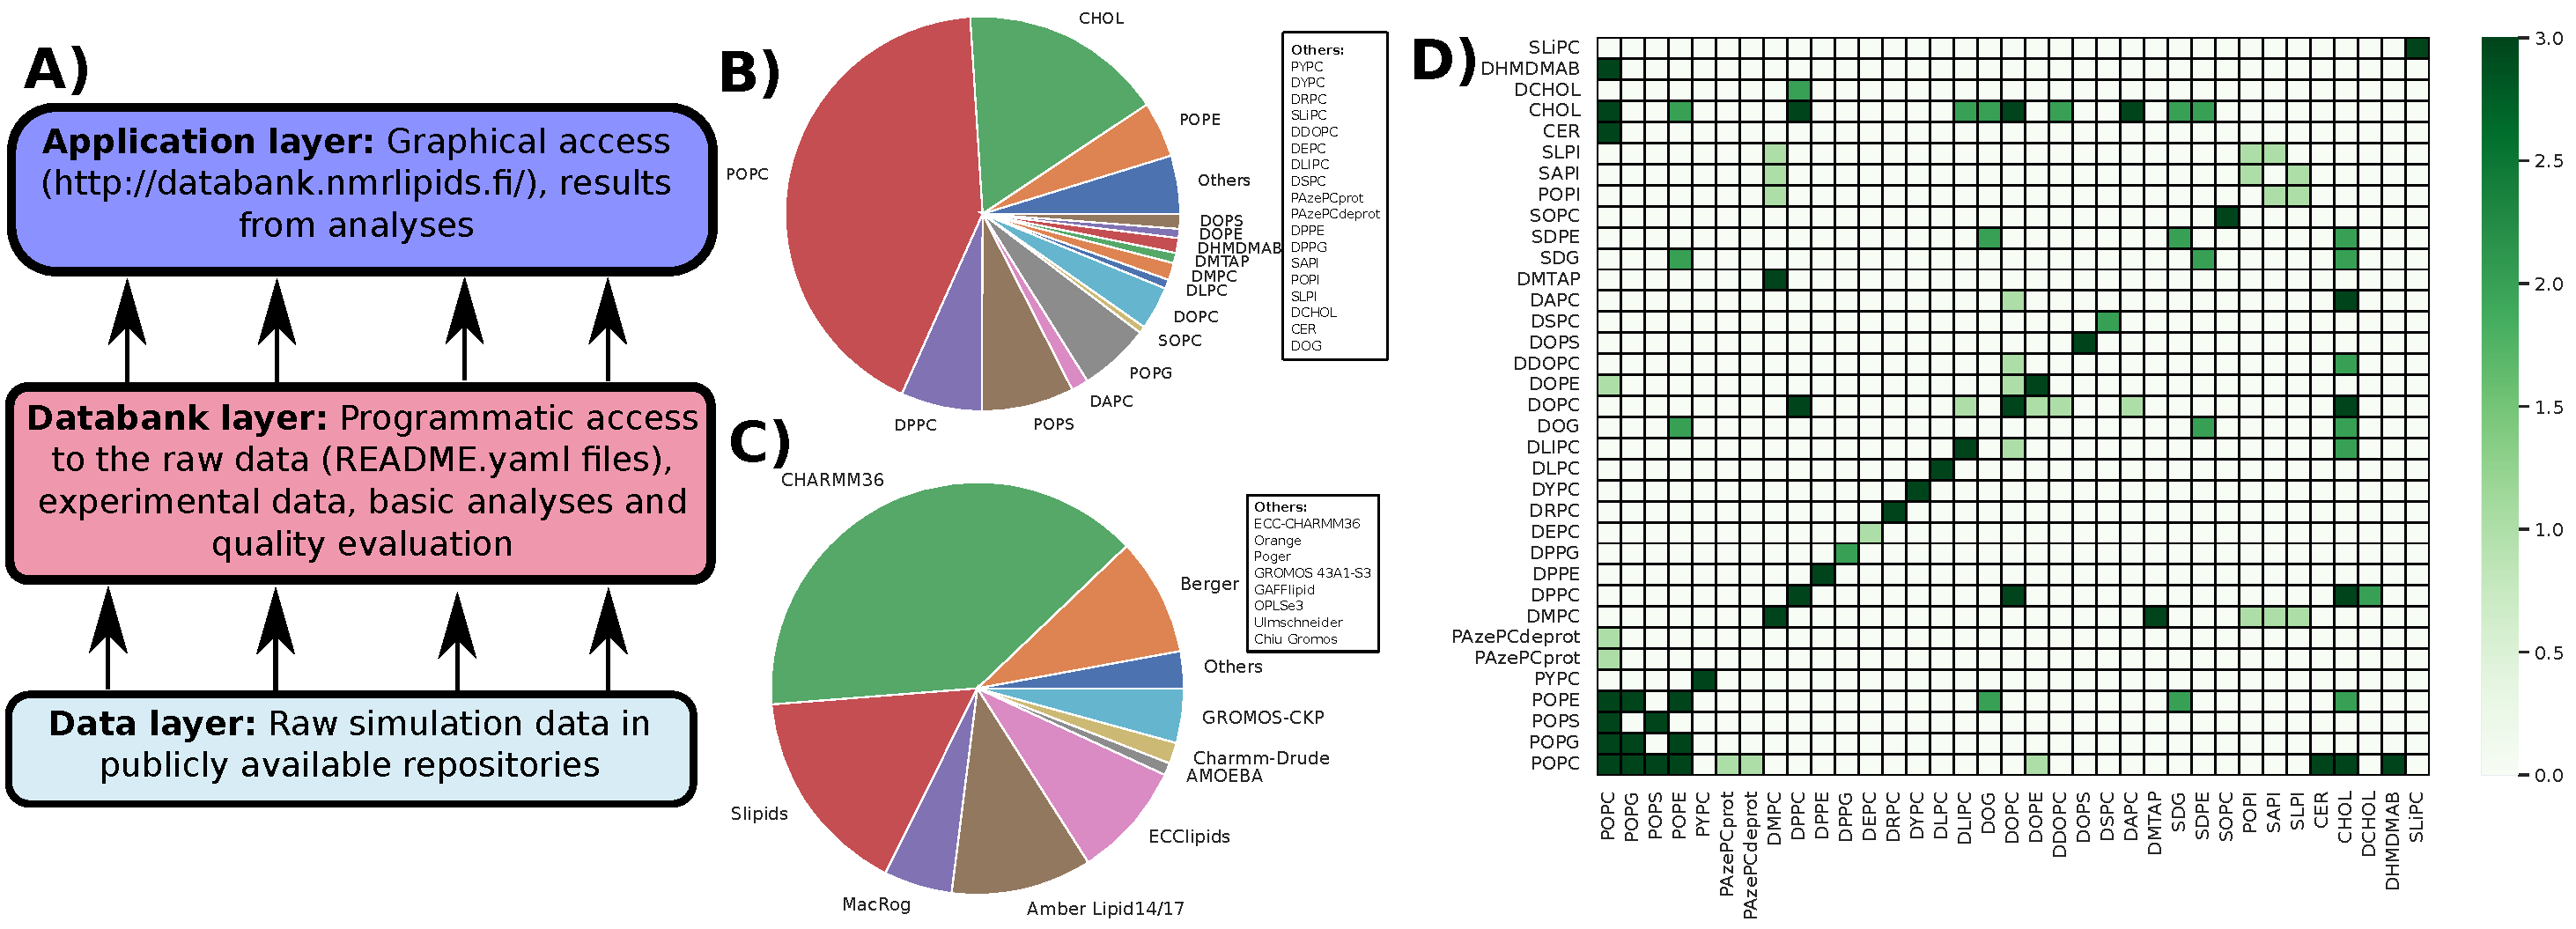
\includegraphics[width=\linewidth]{Figures/overlay3.pdf}
    \caption{Overview of the NMRlipids Databank. 
    \textbf{A} Schematic presentation of the overlay structure used in the NMRlipids Databank. A more detailed structure of the \textit{Databank layer} is shown in Fig.~\ref{DatabankStructure} in the SI.
    \textbf{B} Distribution of lipids present in the trajectories of the Databank. `Others' lists lipids occurring in five or fewer simulations. 
    \textbf{C} Distribution of force fields in the simulations in the Databank. References for each force field are given in Table~\ref{tab:ForceFields}.
    \textbf{D} Flowchart for performing an analysis of properties through all MD simulations in the NMRlipids Databank using the API.
    \textbf{E} Flowchart for accessing results calculated from the NMRlipids Databank and stored to the \textit{Application layer}.
    \textbf{F} Currently available single lipid component and binary mixtures in the NMRlipids Databank. Colorbar shows the number of available simulations with the darkest green indicating three or more.  
    }
    \label{fig:overlay}
\end{figure}

\subsection{NMRlipids Databank-GUI: graphical access to the MD simulation data}
NMRlipids Databank-GUI, available at~\href{https://www.databank.nmrlipids.fi}{databank.nmrlipids.fi}, provides easy access to the NMRlipids Databank content through a graphical user interface (GUI). Simulations can be searched based on their molecular composition, force field, temperature, membrane properties, and quality; the search results are ranked based on the simulation quality as evaluated against experimental data when available. Membranes can be visualized, and properties between different simulations and experiments compared. The NMRlipids Databank-GUI enables rapid surveying of what simulation data is available, selection of the best available simulations for specific systems based on ranking lists, and comparisons of basic properties between different types of membranes. Notably, the GUI enables these operations to be performed by scientists with a wide range of backgrounds---including those who do not necessarily have programming expertise or other means to access MD simulation data. 

\subsection{NMRlipids Databank-API: programmatic access to the MD simulation data}\label{section:access}
The NMRlipids Databank-API, available at \href{https://github.com/NMRlipids/Databank}{github.com/NMRlipids/Databank}, provides programmatic access to all simulation data in the NMRlipids Databank through application programming interface (API). This enables wide range of novel data-driven applications---from construction of machine learning models that predict membrane properties, to automatic analysis of virtually any property across all simulations in the Databank. The flowchart in Fig.~\ref{fig:overlay}D illustrates the practical implementation of such an analysis. After cloning the databank repository to a local computer, raw data of each simulation can be accessed by iterating through the README.yaml files in the {\it Databank layer} that contain links pointing to the locations of simulation trajectories and other relevant files. Simulations can then be automatically analyzed with the help of the README.yaml and the mapping files that associate the specific naming conventions in each simulation with the universal molecule and atom names used by the Databank. Finally, the analysis results are stored using the same structure as in the {\it Databank layer}. Practical examples of codes that utilize the NMRlipids Databank-API, as well as a template for a new analysis, can be found from locations listed in Table~\ref{tab:codes}.

While analysis codes and results for basic membrane properties are included in the {\it Databank layer}, unlimited further analyses can be implemented by anyone in separate repositories in the {\it Application layer}. When {\it Application layer} repositories are organized by mimicking the {\it Databank layer} structure, they can be accessed programmatically and further analyzed using the tools in the NMRlipids Databank-API by implementing the flowchart demonstrated in Fig.~\ref{fig:overlay}E. Novel analyses that demonstrate the power of NMRlipids Databank in selecting the best simulation models, analysing rare phenomena, and extending MD simulations to new fields are implemented in an {\it Application-layer} repository located at~\href{https://github.com/NMRlipids/DataBankManuscript}{github.com/NMRlipids/DataBankManuscript}. The related codes are listed in Table~\ref{tab:codesApplication}.


\subsection{Applications of the NMRlipids Databank}
\subsubsection{Selecting simulation parameters using NMRlipids Databank: Best models for most abundant neutral membrane lipids}
%Quality of membrane simulations with different force fields have been evaluated against experimental data during parameterization and in separate comparison studies~\cite{botan15,ollila16,catte16,pluhackova16,perez17,leonard19,??}, but the lack of universal quality measure for membrane simulations complicates the estimations of reliability of simulations. 
%
%For example, OPLS3e parameters overcome CHARMM36 in structural quality for POPC but predicts overestimated ion binding~\cite{kurki22}. On the other hand, CHARMM36 gives the best description for lipid headgroup conformational ensembles~\cite{bacle21}, while GROMOS-CKP parameters best capture the membrane packing in POPS bilayers~\cite{antila22b}. 
%
To minimize the detrimental consequences of artificial MD simulation results for their applications, the quality of lipid bilayer MD simulations has to be carefully assessed~\cite{antila22b}. This can be done, for example, against the C--H bond order parameters from NMR spectroscopy~\cite{bacle21,Wur23} and the form factors from X-ray scattering~\cite{ollila16}, although it requires comparisons between large number of simulations, which is laborious even with collaborative approaches~\cite{botan15,catte16,antila19,bacle21}. To streamline this process, we have defined quantitative quality measures that enable automatic ranking of lipid bilayer simulations based on their quality against experiments. Conformational ensembles of individual lipid molecules are evaluated in the NMRlipids Databank by first calculating the probabilities for each C--H bond order parameter to locate within experimental error and then averaging the possibilities over different lipid segments ($P^{\mathrm{hg}}$, $P^{\mathrm{sn1}}$,$P^{\mathrm{sn2}}$, and $P^{\mathrm{total}}$). Furthermore, the quality against X-ray scattering experiments ($FF_q$) is estimated as the difference in the experimental and simulated locations of the first form factor minimum. These measures can be used to evaluate membrane dimensions, as the form factor minima locations and acyl chain C--H bond order parameters correlate with the membrane lateral packing and thickness (Figs.~\ref{fig:quality}G,~\ref{fig:QualityCorrelationsSI}, and~\ref{fig:sizedependence}). In addition, the ergodicity of conformational sampling of lipids is estimated by calculating $\tau_\mathrm{rel}$, the convergence time of the slowest principal component divided by the simulation length. Here we demonstrate how the automatic simulation-quality evaluation and the NMRlipids Databank-API enable rapid selection of the best models for simulations of membranes with the two most biologically-abundant neutral membrane lipids~\cite{vanmeer08}: POPC and POPE.

As Fig.~\ref{fig:quality}A illustrates, predictions for the lateral packing of POPC and POPE membranes in terms of area per lipid, one of the most important parameters used to characterize cellular membranes, diverge between different force fields. To select the most realistic currently available force fields to describe POPC--POPE membranes, we first order simulations in the Databank according to their C--H bond order parameter quality ranking (Fig.~\ref{fig:top50simulations}). From these results, we then pick the force fields occurring in Fig.~\ref{fig:quality}A (that is: force fields for which both POPC and POPE simulations exist in the Databank) and rank them according to the quality of the \textit{sn}-1 chain of POPC (Fig.~\ref{fig:quality}B) and of POPE (Fig.~\ref{fig:quality}C). Simulations with $\tau_\mathrm{rel}$ clearly above one (larger than 1.3) are discarded. Because the membrane packing correlates with the average order parameter of the \textit{sn}-1 chain (Fig.~\ref{fig:quality}G), rankings in Figs.~\ref{fig:quality}B and C can be used to select the simulations giving the most realistic results in Fig.~\ref{fig:quality}A. (Figs.~\ref{fig:quality}E--F and~\ref{fig:POPC_POPE_dataSI} also show direct comparisons with the experimental data for the most relevant simulations; for reference, Fig.~\ref{fig:quality}D shows the overall highest-ranked simulation: POPC bilayer with OPLS3e parameters.) Based on these rankings, Lipid17 and Slipids simulations give the most realistic predictions for a POPC membrane, while simulations with CHARMM36 and GROMOS-CKP parameters predict overly packed bilayers (overestimated order in Fig.~\ref{fig:POPC_POPE_dataSI}). For POPE, on the other hand, GROMOS-CKP and Slipids give the most realistic results, while CHARMM36 and Lipid17 predict membranes that are too packed. In conclusion, the quality evaluation based on the NMRlipids Databank suggests that the Slipids parameters are the best currently available choice for simulations with PC and PE lipids, at least for applications where membrane packing is relevant.

\begin{figure}[!t]
    \centering
    \includegraphics[width=\linewidth]{Figures/quality5.pdf}
    \caption{Examples of data obtained using NMRlipids Databank. 
    \textbf{A} Area per lipid of POPC and POPE lipid bilayers predicted by different force fields at 310\,K in simulations that are available in the NMRlipids Databank. The data points from the best-performing simulations, based on rankings in panels B and C, are surrounded by black circles. 
    \textbf{B} Best POPC simulations ranked based on the \textit{sn}-1 acyl chain order parameter quality ($P^\mathrm{sn1}$). Also \textit{sn}-2 acyl chain ($P^\mathrm{sn2}$), headgroup ($P^\mathrm{hg}$) and total ($P^\mathrm{total}$) order parameter qualities, form factor quality ($FF_q$), and relative equilibration time for conformations ($\tau_\mathrm{rel}$) are shown. Note that the best possible order parameter quality is one, while the best possible form factor quality is zero.
    \textbf{C} Best POPE simulations ranked based on the \textit{sn}-1 acyl chain order parameter quality. 
    \textbf{D--F} Direct comparison against experimental (NMR order parameters and X-ray scattering ) data exemplified for a simulation with the best overall order parameter quality (D), the best quality for POPE lipid (E), and the headgroup quality for POPE (F).
    \textbf{G} Scatter plots and Pearson correlation coefficients, $r$, for the membrane area per lipid, thickness, first minimum of X-ray scattering form factor and average order parameter of the \textit{sn}-1 acyl chain extracted from the NMRlipids Databank. All correlation coefficients have p-value below 0.001. For more correlations see Fig.~\ref{fig:QualityCorrelationsSI}.
    }
    \label{fig:quality}
\end{figure}

\subsubsection{Detecting rare phenomena using NMRlipids Databank: Cholesterol flip-flops}
Lipid flip-flops from one bilayer leaflet to another play an important role in lipid trafficking and regulating membrane properties~\cite{vanmeer08}. Phospholipid flip-flop events are rare when not facilitated by proteins, occurring spontaneously on the timescale of hours or days, while cholesterol, diacylglycerol, and ceramide flip-flop much more often. Still, the reported timescales range from minutes to sub-millisecods~\cite{vanmeer08,steck12,parisio16,gu19}. These timescales were previously accessible only by coarse-grained simulations or free energy calculations~\cite{parisio16}, and atomistic simulations reporting cholesterol flip-flop events have been published only recently~\cite{gu19,javanainen19,baral20}. The atomistic studies report an increase in cholesterol flip-flop rates with increasing acyl chain unsaturation level and decreasing cholesterol concentration~\cite{gu19,javanainen19}, but the amount of data in these individual studies was not sufficient to systematically assess correlations between cholesterol flip-flop rates and membrane properties. Here, we demonstrate that the NMRlipids Databank-API makes analyses of such rare phenomena accessible for all by enabling access to a large amount of MD simulation data as illustrated in Fig.~\ref{fig:overlay}. This is particularly useful for scientists in various fields of science and industry who lack access to the computational resources or the expertise to produce the large amounts of MD simulation data required for such analyses. 


Using the general workflow depicted in Fig.~\ref{fig:overlay}D, we first calculated the flip-flop rates from all the simulations available in the NMRlipids Databank. Flip-flops were observed for cholesterol, DCHOL (18,19-di-nor-cholesterol), DOG (1,2-dioleoyl-\textit{sn}-glycerol), and SDG (1-stearoyl-2-docosahexaenoyl-\textit{sn}-glycerol). The observed cholesterol flip-flop rates, ranging between 0.001--1.6\,\textmu{}s$^{-1}$ with the mean of 0.16\,\textmu{}s$^{-1}$ and median of 0.07\,\textmu{}s$^{-1}$, are in line with the previously reported values from atomistic MD simulations~\cite{gu19,javanainen19,baral20}. The flip-flop rate of DCHOL, 0.2\,\textmu{}s$^{-1}$, was close to the average value of cholesterol, while the average rates for diacylglycerols DOG (0.4\,\textmu{}s$^{-1}$) and SDG (0.5\,\textmu{}s$^{-1}$) were higher than for cholesterol. Flip-flops were not observed for other lipids, giving the upper limits for PC-lipid flip-flop rate as 9$\times$10$^{-6}$\,\textmu{}s$^{-1}$ and for ceramide (\textit{N}-palmitoyl-\textsc{D}-\textit{erythro}-sphingosine) as 0.002\,\textmu{}s$^{-1}$. Thus, the available data in the NMRlipids Databank suggest that the lipid flip-flop rate decreases in the order: diacylglycerols $>$ cholesterol $>$ other lipids including ceramides. However, the amount of data for diacylgycerols (8 simulations with the Lipid17 force field) and ceramide (3 simulations with CHARMM36) is less than that for cholesterol (83 simulations); thus we cannot fully exclude the effect of force field or composition on this comparison.

Nevertheless, we used the general workflow depicted in Fig.~\ref{fig:overlay}E to analyse how the flip-flop rates calculated from the NMRlipids Databank depend on membrane properties. Figures~\ref{fig:flip-flops}B--D show cholesterol flip-flop rates and their histograms as a function of membrane thickness, lateral density, and acyl chain order. The results reveal a non-linear correlation between cholesterol flip-flop rate and membrane packing (depicted as area per lipid): Flip-flop rates increase by an order of magnitude when membrane packing density decreases, and a major jump is observed at low membrane packing. Such order-of-magnitude changes in cholesterol flip-flop rate with the membrane composition may have major implications in understanding lipid trafficking and membrane biochemistry~\cite{gu19,baral20}. Because the results from the NMRlipids Databank are averaged over a large range of membrane compositions and force fields, they show that the strong dependence of cholesterol flip-flop rate on membrane properties is not limited to the particular lipid compositions or force fields used in the previous studies~\cite{gu19,javanainen19,baral20}.

\begin{figure}[htb]
    \centering
    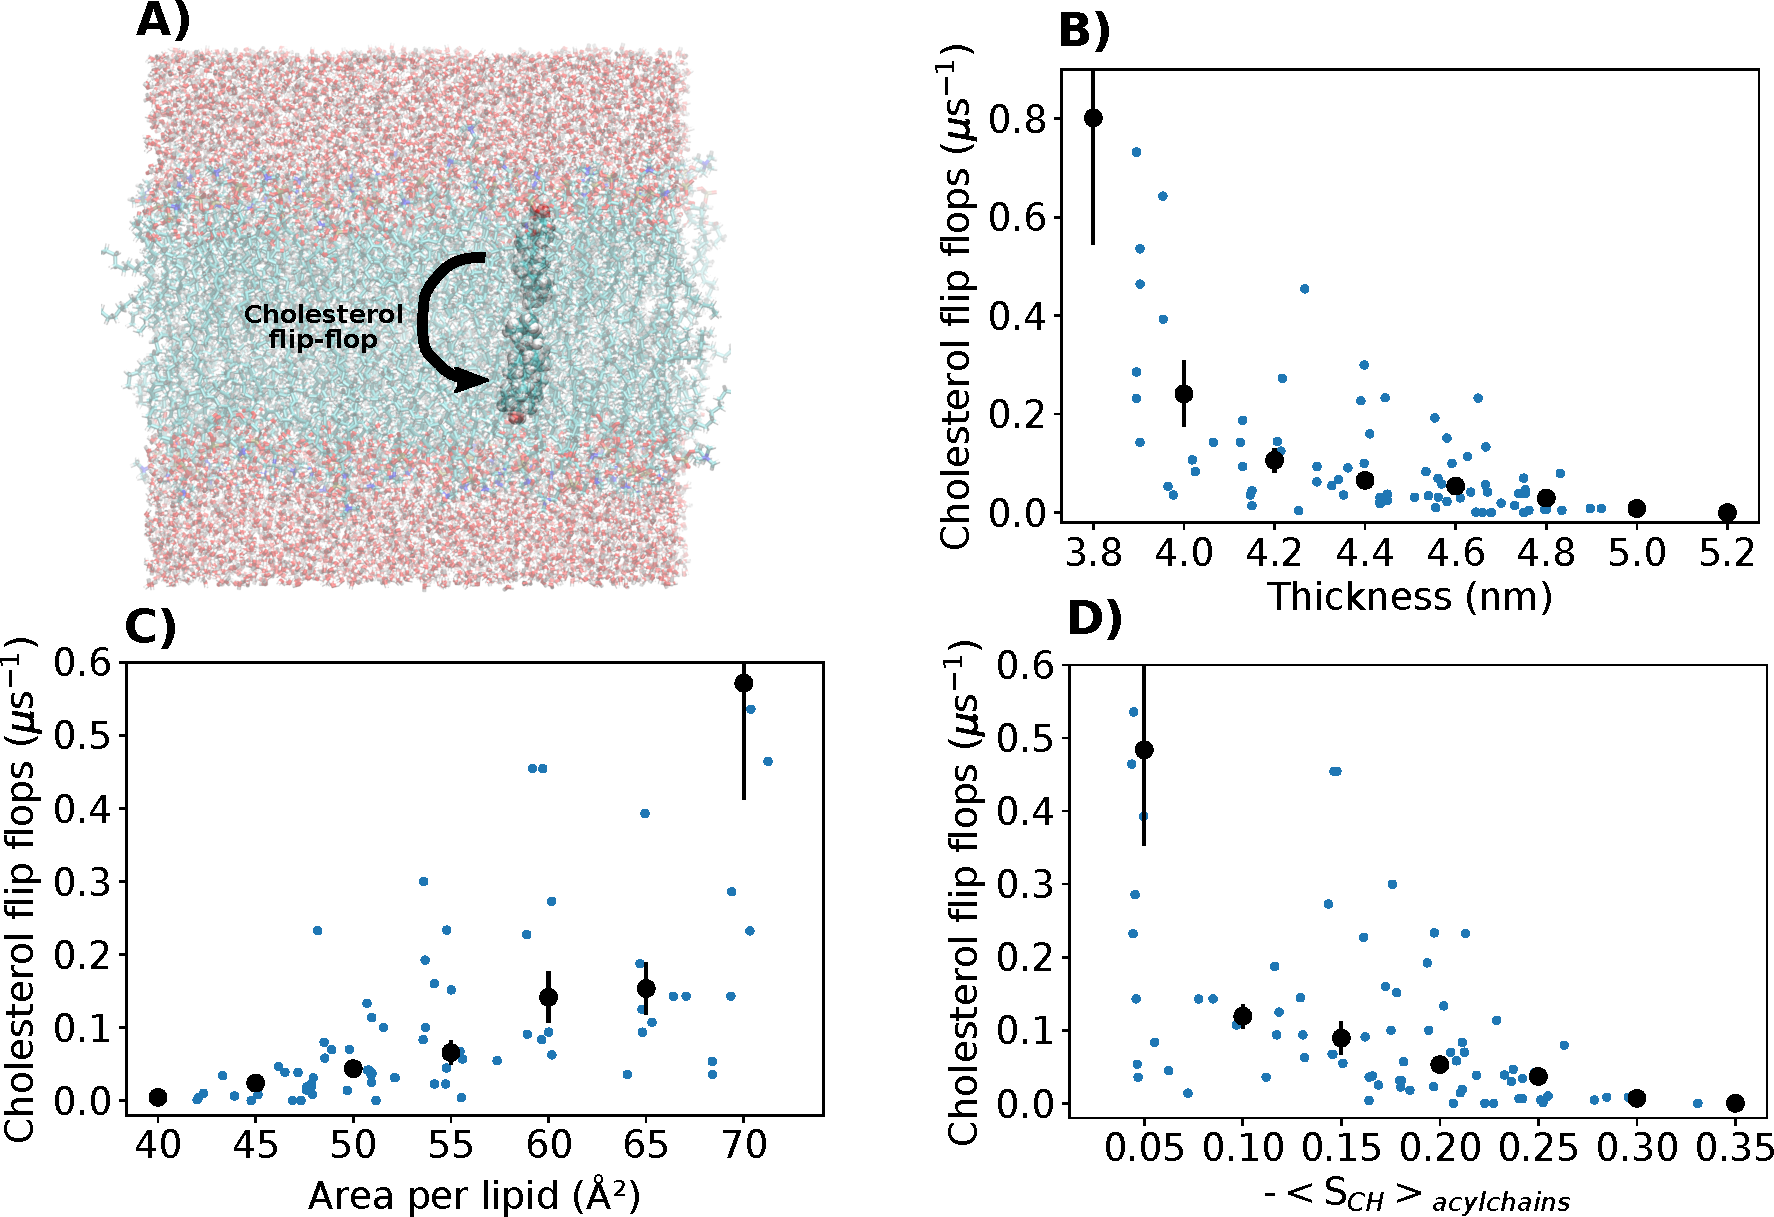
\includegraphics[width=88mm]{Figures/CholFlipFlops.pdf}
    \caption{Quantification of cholesterol flip-flop events in NMRlipids Databank simulations. 
    \textbf{A} Illustration of cholesterol flip-flop.  
      \textbf{B--D} Cholesterol flip-flops analyzed from the Databank as a function of membrane thickness, area per lipid, and acyl chain order. Values from simulations with non-zero flip-flop rates are shown with blue dots. Histogrammed values are shown with black dots. For the mean value in each bin, average weighted with the simulation lengths was used, and error bars show the standard error of the mean.
    }
    \label{fig:flip-flops}
\end{figure}



\subsubsection{Extending the scope of MD simulations to new fields using NMRlipids Databank: Water diffusion anisotropy in membrane systems}
The anisotropy of water diffusion in directions parallel and perpendicular to membranes can be related to translocation of drugs through biological material, particularly in the skin \cite{hansen13,wen18,nitsche19,roberts21}, and to signal formation in diffusion tensor MRI imaging~\cite{topgaard20}. MD simulations are rarely used to analyze the anisotropic diffusion of water, since only a few membrane permeation events of water are typically observed in a single MD simulation trajectory~\cite{venable19,camilo2022}, thereby making the collection of a sufficient amount of data challenging. Here, we show that the API access to the data in NMRlipids Databank enables systematic analysis on how the anisotropic diffusion of water depends on membrane properties in multilamellar membrane systems, thereby extending the application of MD simulations to new fields. 

\begin{figure}[tb]
    \centering
    \includegraphics[width=\linewidth]{Figures/permeation3.pdf}
    \caption{Quantification of water diffusion in NMRlipids Databank simulations.
    \textbf{A} Water diffusion, $D_\perp$, and permeability, $P$, through membranes, and lateral diffusion along the membrane, $D_\parallel$, illustrated in a multilamellar stack of lipid bilayers. 
    \textbf{B--E} Water permeation through membranes analyzed from the Databank as a function of temperature, thickness, area per lipid, and acyl chain order. Inset in B) shows the Arrhenius plot of permeation ($\ln(P)$ vs. $1/T$) that gives 14\,$\pm$\,3\,$k_\mathrm{B}T$ for the average activation energy for water permeation through lipid bilayer. 
    \textbf{F} Lateral diffusion of water as a function of hydration level. Experimental points for DMPC bilayers at 313\,K at different hydration levels are shown~\cite{rudakova04}.
    \textbf{G--H} Diffusion anistoropy of water as a function of thickness and area per lipid. 
    Non-zero permeation and diffusion values from simulations are shown with blue dots. Histogrammed values are shown with black dots. For the mean value in each bin, average weighted with the simulation lengths was used, and error bars show the standard error of the mean. Only bins with more than one microsecond of data in total were used for water permeation.}
    \label{fig:permeability}
\end{figure}


To this end, we first calculated the water permeability through membranes from all simulations in the NMRlipids Databank using the general workflow depicted in Fig.~\ref{fig:overlay}D. The resulting non-zero values range between 0.3--322\,\textmu{}m/s with the mean of 14\,\textmu{}m/s and median of 8\,\textmu{}m/s. These values agree with the previously reported simulation results~\cite{venable19,camilo2022}, but are on average larger than experimental values reported for PC lipids in the liquid crystalline phase,~0.19--0.33\,\textmu{}m/s~\cite{jansen95}. Using the workflow depicted in Fig.~\ref{fig:overlay}E, we then plotted the observed permeabilities and their histogrammed values in Figs.~\ref{fig:permeability}B--E as a function of temperature, membrane thickness, area per lipid, and acyl chain order. As expected, the permeability increases with the temperature, giving an average energy barrier of 14\,$\pm$\,3\,$k_\mathrm{B}T$ for the water permeation from the Arrhenius plot in Fig.~\ref{fig:permeability}B. On the other hand, the water permeability on average decreases when membranes become more packed, that is, with decreasing area per lipid and increasing thickness and acyl chain order (Figs.~\ref{fig:permeability}C--E). Permeation of water through bilayers depends on membrane properties also according to previous studies, but there is no established consensus on whether the area per lipid~\cite{nagle08} or bilayer thickness~\cite{frallicciardi22} is the main parameter determining the permeability. 
%is previously reported from simulations and experiments for some systems, but not for all~\cite{mathai07,venable19,frallicciardi22}. 
Our analysis over the NMRlipids Databank, containing significantly more data than what was available in previous studies, suggest non-linear dependencies on both of these parameters.
%, yet the linear correlation would be a good approximation for thicknesses $\gtrsim$\,3.9\,nm and area per lipids $\lesssim$\,69\,\AA{}$^2$ (insets in Figs.~\ref{fig:permeability}C--D).
%within the range of experimentally reported values  permeability which is 1-2 orders of magnitude slower than osmotic permeability \cite{jansen95,??}. 
Clear dependencies of permeability on hydration level or the fraction of charged lipids, cholesterol, or POPE in the membrane were not observed (Fig.~\ref{fig:permeationSI}).
%
%%Several models on how water dynamics depends on membrane properties have been proposed~\cite{mathai07,nitsche13,nitsche16,shinoda16,venable19,frallicciardi22}.  


To examine how water diffusion anisotropy depends on membrane properties in a multi-lamellar lipid bilayer system, we analyzed the water diffusion parallel to the membrane surface from all simulations in the NMRlipids Databank using the general workflows depicted in Figs.~\ref{fig:overlay}D and E. The parallel diffusion coefficient of water, $D_\parallel$, decreases with reduced hydration and increases with the temperature, but dependencies on the membrane area per lipid, thickness, or fraction of charged lipids were not observed in Figs.~\ref{fig:permeability} and~\ref{fig:diffusionSI}. Simulation results are close to the experimental values with low hydration levels in Fig.~\ref{fig:permeability}F, but increase to approximately 50\% higher than the experimental value for bulk water diffusion value (3.1$\times$\,10$^{-9}$\,m$^2$/s at 313\,K~\cite{khakimov08}) with high hydration levels.
This is not surprising as the most common water model used in membrane simulations, TIP3P, overestimates the bulk water diffusion~\cite{pathirannahalage21}. To estimate the diffusion anisotropy of water, $D_\perp/D_\parallel$, in multilamellar membrane system, the permeability coefficients of water through membranes were translated to perpendicular diffusion coefficients, $D_\perp$, using the Tanner equation~\cite{tanner78,wasterby02}. The resulting perpendicular diffusion coefficients are approximately five orders of magnitude smaller than the lateral diffusion coefficients of water (Figs.~\ref{fig:permeability}G--H), which is at the upper limit of anisotropy estimated from experimental data~\cite{nitsche19}. A significant increase in the diffusion anisotropy with membrane packing is observed, as $D_\perp/D_\parallel$ deviates further from unity with decreasing area per lipid and increasing thickness in Figs.~\ref{fig:permeability}G--H. This follows from decreasing water permeability with membrane packing (Figs.~\ref{fig:permeability}C--D), while lateral diffusion remains approximately constant (Figs.~\ref{fig:diffusionSI}A,~C).

In summary, our results suggest that the bilayer packing has a substantial effect on anisotropic water diffusion in multi-membrane lipid systems. The several-fold larger anisotropy in membranes with higher lateral density is expected to play a role in pharmacokinetic models not only for water but also for other hydrophilic molecules~\cite{nitsche19}. Furthermore, the enhanced understanding of this anisotropy may help in developing new diffusion-tensor-based MRI imaging methods where signals originate from the anisotropic diffusion of water in biological matter~\cite{topgaard20}.

\section{Discussion}

%The Discussion should be succinct and must not contain subheadings.

The focus of biomolecular simulations is moving from studies of individual molecules to larger complexes and even whole cells and organelles~\cite{johnson15,thornburg22,gupta22}. Simultaneously, machine-learning-based models for predicting the behaviour of biomolecules and automatic approaches to parametrize models are emerging~\cite{jumper21,antila22b}. The resources delivered by the NMRlipids Databank will support the development in both of these directions. Automatic quality evaluation and ranking of simulations against experimental data enable the selection of best simulations for specific applications without laborious manual force field evaluation. This also streamlines automatic parametrization procedures for atomistic and coarse grained simulations by, for example, pinpointing typical failures of force fields and highlighting points of improvement. Such practises for fostering the accuracy of simulations are becoming increasingly important due the accumulation of small errors when complexity and size of simulated systems are increasing.

The open programmatic access to unprecedented amounts of MD simulation data through the NMRlipids Databank-API enables a wide range of novel data-driven analyses and machine learning applications. The analyses of cholesterol flip-flop events (Fig.~\ref{fig:flip-flops}) and water permeation through membranes (Fig.~\ref{fig:permeability}) demonstrate how a large amount of accessible simulation data in terms of quantity (\textit{e.g.}, simulation length and number of conformations) and content (\textit{e.g.}, lipid compositions and ion concentrations) enable analyses of rare phenomena that are beyond the current possibilities for a single research group. Such analyses also pave the way for applications of MD simulations in new fields, as demonstrated here by analysing an essential parameter in pharmacokinetic modeling and MRI imaging:\cite{nitsche19,topgaard20} the anisotropic diffusion of water in membrane systems (Fig.~\ref{fig:permeability}). Furthermore, the NMRlipids Databank-API delivers access to a training set data that paves the way for diverse machine learning applications to predict membrane properties. Such applications could be analogous to AlphaFold \cite{jumper21} and other tools~\cite{baek21,lin23} that predict protein structures from their sequence using artificial intelligence. These possibilities are particularly valuable for scientists who do not typically have access to large scale MD simulation data. Expected applications of the NMRlipids Databank in a wide range of fields are listed in Table~\ref{tab:applications}, yet the scope of such applications
%in biology, biotechnology, material science, biomolecular imaging and beyond
is expected to further widen with increasing amount of data in the Databank.  


\begin{table}[t]
    \centering
    \begin{tabular}{p{5.0cm}  p{5.0cm}  p{4.0cm}}
    Type of application     & Practical examples & Target group \\
    \hline
    Analyses of rare phenomena               & Lipid flip-flops, water permeation (Figs.~\ref{fig:flip-flops} and~\ref{fig:permeability}) & Membrane scientists \\
    \\
    Correlations between membrane properties & 
    Membrane structural properties, water dynamics (Figs.~\ref{fig:quality} and~\ref{fig:permeability}) & 
    Membrane scientists \\
    \\
    Applications that are outside the typical scope of MD simulations & 
    Anisotropic water diffusion for pharmacokinetics and MRI imaging applications (Fig.~\ref{fig:permeability}) & 
    Scientists in fields where MD simulations are not usually applied \\
    \\
    Selection of the best simulation model for a specific application & 
    Best model for membranes with PC and PE lipids (Fig.~\ref{fig:quality}), lipid headgroup conformations~\cite{bacle21}, 
    packing of PS~\cite{antila22b} and PE (Fig.~\ref{fig:quality}) containing membranes &
    Scientists using MD simulations \\
    \\
    Guidance for force field development & 
    Improvements in ion binding to lipids~\cite{melcr18,melcr20} and lipid headgroup conformational ensembles~\cite{yu21,dickson22,grote20} &
    Scientists developing parameters for MD simulations \\
    \\
    Training and target data for the development of coarse grained models & 
    Optimizing parameters of coarse grained models against NMRlipids Databank, extracting continuum parameters for membranes &
    Scientists developing and using coarse grained MD simulations \\
    \\
    Training set for machine learning applicatons &
    Programmatic access to the data and results enables training of machine learning models for various applications, such as predictions of membrane properties from composition & Scientists building and using machine learning applications for biomolecules
    \end{tabular}
    \caption{Examples on applications of the NMRlipids Databank.}
    \label{tab:applications}
\end{table}

Potential benefits of sharing MD simulation data are widely recognized by different stakeholders from scientists~\cite{feig99,tai04,silva06,abraham19,hildebrand19,hospital20,abriata20,espigares20} to funders and journal staff, but data sharing with efficient tools for upcycling have been rare. The main barriers for such solutions have been the required commitment for the long term support of hardware and software, and the lack of incentives for researchers to share the data. The first issue is solved in the NMRlipids Databank by the overlay design, where the raw data is distributed to already publicly available decentralized locations, while the core of the Databank is composed only of the metadata stored in a version-controlled git repository with an open-access license. On the other hand, the open collaboration approach developed in the NMRlipids Project~\cite{botan15} creates incentives for sharing the data by offering authorship in published articles to the contributors. Advantages of such an approach are demonstrated here for membrane simulations, but the concept can be applied not only to other biomolecules, such as disordered proteins and membrane--protein systems, but also in other fields where similar barriers hinder the machine learning revolution, such as the assignment of NMR spectra~\cite{klukowski22}. 



\newpage


\section{Methods}

%Topical subheadings are allowed. Authors must ensure that their Methods section includes adequate experimental and characterization data necessary for others in the field to reproduce their work.

\subsection{Structure of the Databank}
The overlay structure designed for the NMRlipids Databank is composed of three layers (Fig.~\ref{fig:overlay}A). The {\it Data layer} contains raw data that can be distributed to publicly available servers such as Zenodo (\href{https://www.zenodo.org/}{zenodo.org}). The core content of the Databank locates in the {\it Databank layer}, which is a git repository at \href{https://github.com/NMRlipids/Databank/}{github.com/NMRlipids/Databank} and is also permanently stored in a Zenodo repository (\href{https://www.zenodo.org/}{zenodo.org})~\cite{??}. The essential information of each simulation is stored in a human-and-machine-readable README.yaml file located in a subfolder of the \texttt{/Data/Simulations} folder in the {\it Databank layer} repository; each subfolder has a unique name constructed based on a hash code of the trajectory and topology files of each simulation. The README.yaml files in these folders contain access to all information that is needed for further analysis of simulations, such as links to the raw data and associations with the universal molecule and atom names. The content of these files is described in detail in Table~\ref{tab:READMEkeys} in the supplementary information. Results from analyses of basic membrane properties (area per lipid, thickness, C--H bond order parameters, X-ray scattering form factors, and relaxation of principal components) are stored in the same folders as the README.yaml files. Experimental data used for ranking is stored in the \texttt{/Data/experiments} folder, the ranking results in \texttt{/Data/Ranking}, and the relevant scripts in the \texttt{/Scripts/} folder in the {\it Databank layer} repository. The scripts in the NMRlipids Databank are mainly written in Python and many of them use the MDAnalysis module~\cite{gowers2019mdanalysis,michaud2011mdanalysis}. The Databank structure is illustrated in more detail in Fig.~\ref{DatabankStructure} in the supplementary information. Whenever specific files or folders are referred here, they locate at the {\it Databank layer} repository unless stated otherwise. 

\subsection{Universal naming convention for molecules and atoms} \label{naming}
When analysing simulation trajectories, atoms and molecules often need to be  called by the names used in the trajectory. However, these names typically vary between force fields, as a universal naming convention has not been defined for lipids. To enable automatic analyses over all the simulations in the NMRlipids Databank, we have defined universal naming conventions for the molecules and atoms therein. The universal abbreviations used in the NMRlipids Databank for each molecule are listed in Table~\ref{tab:abbreviations} in the supplementary information. The atom names used in simulation trajectories are connected to the universal atom names using the mapping files defined in the NMRlipids Project (\url{https://nmrlipids.blogspot.com/2022/04/new-yaml-format-of-mapping-files.html}). These files are located at \texttt{/Scripts/BuildDatabank/mapping\_files} in the NMRlipids Databank repository. These files also define whether an atom belongs to the headgroup, glycerol backbone, or acyl chain region in a lipid. In practise, the force-field-specific molecule names and mapping file
names are given in the COMPOSITION dictionary in the README.yaml files for each molecule in each simulation in the NMRlipids Databank.

\subsection{Adding data to NMRlipids Databank}
The NMRlipids Databank is open for additions of simulation data by anyone. The list of information that a contributor has to deliver is given in Table~\ref{tab:READMEkeys}. The rest of the information to be stored in the README.yaml files, also listed in Table~\ref{tab:READMEkeys}, will be automatically extracted using the \texttt{/Scripts/BuildDatabank/AddData.py} script. In practise, the manually entered data is first stored into an info.yaml file that is then added to the \texttt{/Scripts/BuildDatabank/info\_files} folder trough a git pull request. To avoid ineligible entries and minimize human errors, the pull requests are monitored before the acceptance and generation of the README.yaml files.  Currently, the NMRlipids Databank is composed of simulations that are found from the Zenodo repository with an appropriate license; most, but not all, of these trajectories originate from previous NMRlipids projects~\cite{botan15,catte16,antila19,bacle21}.


\subsection{Experimental data}
Experimental data used in the quality evaluation, currently composed of C--H bond order parameters and X-ray scattering form factors, are stored in \texttt{/Data/experiments} in the NMRlipids Databank repository. Similarly to simulations, each experimental data set has a README.yaml file containing all the relevant information about the experiment. The keys and their descriptions for the experimental data are given in Table~\ref{tab:READMEkeysEXP}. The NMR data currently in the NMRlipids Databank are taken from Refs.~\citenum{scherer87,ferreira13,antila19,melcr20,bacle21} and the X-ray scattering data from Refs.~\citenum{Kucerka08a,kucerka11,pan12b,pan14,kucerka15,NMRlipidsIII}. In addition, previously unpublished NMR data for POPE, POPG, and DOPC was acquired as described in the supplementary information (Figs.~\ref{POPEexp1}--\ref{fig:DOPCexp}) and contributed to the Databank. 


\subsection{Analysing simulations}
In practise, simulations in the NMRlipids Databank can be analyzed by executing a program that
1) loops over the README.yaml files in the {\it Databank layer},
2) downloads the data using the information in the README.yaml files, and then
3) performs the desired analysis on a local computer utilising the universal naming conventions for molecules and atoms defined in the README.yaml and mapping files.
This general procedure is illustrated in Fig.~\ref{fig:overlay}D, and practical examples of codes that perform such analyses are listed in Tables~\ref{tab:codes} and~\ref{tab:codesApplication}. The equilibration period given by the user (TIMELEFTOUT in Table~\ref{tab:READMEkeys}) is discarded from the trajectories in all analysis codes.


\subsection{Principal Components Analysis of equilibration of simulations}
To estimate how well conformational ensembles of lipids are converged in trajectories, the Principal Component Analysis (PCA) following the PCALipids protocol was used \cite{buslaev16,buslaev2020principal}. 
%, the lipids of a specific type were first selected, and trajectories of individual lipids were concatenated. 
To this end, each lipid configuration was first aligned to the average structure of that lipid type, and PCA analysis was then applied on the Cartesian coordinates of all heavy atoms of the lipid. Because the motions along the first, major, principal component are the slowest ones \cite{buslaev16}, the equilibration of each lipid type was estimated from the ratio between the distribution convergence of the trajectories projected on the first PC and the trajectory length, $\tau_{\rm rel} = \tau_{\text{convergence}}/\tau_{\text{sim}}$~\cite{buslaev16, buslaev2020principal}. If $\tau_{\rm rel} < 1$, simulations can be considered to be sufficiently long for the lipid molecules to have sampled their conformational ensembles, while in simulations with $\tau_{\rm rel} > 1$ individual molecules may not have fully sampled their conformational ensembles. Rigid molecules that do not exhibit significant conformational fluctuations, such as sterols, were excluded from the analysis. 
%The suggested way to estimate the characteristic timescales needed to adequately sample the configurational space of individual lipids is to calculate the distribution convergence of the trajectories projected on the first PC\cite{buslaev16}. 
In practise, the distribution convergence times were calculated utilising its linear dependence on autocorrelation decay times,
%\begin{equation}
    $\tau_{\text{convergence}} = k\tau_{\text{autocorrelation}}$,
%\end{equation}
because calculation of autocorrelation decay times is faster and computationally more stable than direct calculation of distribution convergence times~\cite{buslaev16, buslaev2020principal}. The empirical coefficient $k = 49$ was calculated based on the analysis of 8 trajectories with the length of more than 200\,ns, including simulations of POPC, POPS, POPE, POPG, and DPPC with the CHARMM36 force field. %All simulations, used for $k$ calculation, were at least 200 ns long. 
Because the coefficient $k$ does not depend on the force field~\cite{buslaev16}, the value determined from these CHARMM36 simulations can be used for all simulations in the Databank. The script that calculates the equilibration of lipids is available at \texttt{Scripts/BuildDatabank/NMRPCA\_timerelax.py} in the NMRlipids Databank repository. The resulting values are stored in files named \texttt{eq\_times.json} at folders in \texttt{/Data/Simulations} in the NMRlipids Databank repository. 

\subsection{Calculation of C--H bond order parameters}
The C--H bond order parameters were calculated directly from the carbon and hydrogen positions using the definition
\begin{equation}\label{OP}
S_{\rm CH}=\frac{1}{2}\left\langle 3\cos^2\theta -1 \right\rangle,
\end{equation}
where angular brackets denote the ensemble average, \textit{i.e.}, average over all sampled configurations of all lipids in a simulation, and $\theta$ is the angle between the C--H bond and the membrane normal. As in previous NMRlipids publications, the order parameters were first calculated separately for each lipid and the standard error of the mean over different lipids was used as the error estimate~\cite{botan15}. However, order parameters for simulations with $\tau_{\rm rel} > 1$ may be influenced by the starting structure and thereby their error bars may be underestimated. The script that calculates C--H bond order parameters from all simulations in the NMRlipids Databank is available at \texttt{/Scripts/AnalyzeDatabank/calcOrderParameters.py} in the NMRlipids Databank repository. The resulting order parameters are stored for all simulations in files named %\newline 
[\texttt{lipid\_name}]\texttt{OrderParameters.json} at folders in \texttt{/Data/Simulations} in the NMRlipids Databank repository.

\subsection{Calculation of X-ray scattering form factors}
X-ray scattering form factors were calculated using the standard equation for lipid bilayers that does not assume symmetric membranes~\cite{ollila16},
\begin{equation}\label{FFsimpl}
F(q)= \left\lvert\int_{-D/2}^{D/2}\Delta \rho_e(z) \exp(\iu zq_z) {\rm d}z \right\rvert,
\end{equation}
where $\Delta \rho_e(z)$ is the difference between the total and solvent electron densities, and $D$ is the simulation box size in the $z$-direction (normal to the membrane). For the calculation of density profiles, atom coordinates were first centred around the centre of mass of lipid molecules for every time frame, and a histogram of these centred positions, weighted with the number of electrons in each atom, was then calculated with the bin width of $1/3$~\AA{}. Electron density profiles were then calculated as an average of these histograms over the time frames in simulations. The script to calculate form factors for all simulations in the NMRlipids Databank is available at \texttt{Scripts/AnalyzeDatabank/calc\_FormFactors.py}. The resulting form factors are stored for all simulations in files named \texttt{FormFactor.json} at folders in \texttt{/Data/Simulations} in the NMRlipids Databank repository.

\subsection{Calculation of area per lipid and bilayer thickness}
Area per lipids of bilayers were calculated by dividing the time-averaged area of the simulation box with the total number of lipids and surfactant molecules in the simulation (see Table~\ref{tab:abbreviations} for the list of molecules considered as lipids or surfactants). The script that calculates the area per lipid from all simulations in the NMRlipids Databank repository is available at \texttt{Scripts/AnalyzeDatabank/calcAPL.py} in the NMRlipids Databank repository. The resulting area per lipids are stored for all simulations in files named \texttt{apl.json} at folders in \texttt{/Data/Simulations}. 

Thicknesses of lipid bilayers were calculated from the intersection points of lipid and water electron densities. The script that calculates the thicknesses of all simulations in the NMRlipids Databank is available at \texttt{Scripts/AnalyzeDatabank/calc\_thickness.py} in the NMRlipids Databank repository. The resulting thicknesses are stored in files named \texttt{thickness.json} at folders in \texttt{/Data/Simulations} in the NMRlipids Databank repository. 

\subsection{Quality evaluation of C--H bond order parameters}
As the first step to evaluate simulation qualities against experimental data, a simulation is connected to an experimental data set if the molar concentrations of all molecules are within $\pm$3 percentage units, charged lipids have the same counterions, and temperatures are within $\pm$2\,K. For molar concentrations of water, the exact hydration level is considered only for systems with molar water-to-lipid ratio below 25, otherwise the systems are considered as fully hydrated. In practise, the connection is implemented by adding the experimental data path into the simulation README.yaml file using the \texttt{/Scripts/BuildDatabank/searchDATABANK.py} script in the NMRlipids Databank repository. 

The quality of each C--H bond order parameter is estimated by calculating the probability for a simulated value to locate within the error bars of the experimental value. Because conformational ensembles of individual lipids are assumed to be independent in a fluid lipid bilayer, $\frac{S_\mathrm{CH}-\mu}{s/\sqrt{n}}$ has a Student's t-distribution with $n-1$ degrees of freedom and $\mu$ representing the real mean of the order parameter. The probability for an order parameter from simulation to locate within experimental error bars can be estimated from equation
\begin{equation}\label{probability}
  P = f \left( \frac{S_\mathrm{CH} - (S_\mathrm{exp}+\Delta S_\mathrm{exp})}{s/\sqrt{n}} \right) - f \left( \frac{S_\mathrm{CH} - (S_\mathrm{exp}-\Delta S_\mathrm{exp})}{s/\sqrt{n}} \right),
\end{equation}
where $f(t)$ is the %first order 
Student's t-distribution, $n$ is the number of independent sample points for each C--H bond (which equals the number of lipids in a simulation), $S_\mathrm{CH}$ is the sample mean from Eq.~\eqref{OP}, $s$ is the variance of $S_\mathrm {CH}$ calculated over individual lipids, $S_\mathrm{exp}$ is the experimental value, and $\Delta S_\mathrm{exp}$ its error. The error of $\Delta S_\mathrm{exp} = 0.02$ is currently assumed for all experimental order parameters~\cite{ollila16}, yet more accurate ones may be available in the future~\cite{wurl22}. Because a lipid bilayer simulation contains at least dozens of lipids, the Student's t-distribution could be safely approximated with a normal distribution. However, with the quality of currently available force fields, the simulation values can be so far from experiments that a normal distribution leads to probability values below the numerical accuracy of computers. To avoid such numerical instabilities, we opted to use the first order Student's t-distribution that has slightly higher probabilities for values far away from the mean. On the other hand, some force fields exhibit too slow dynamics, which leads to large error bars in the $S_\mathrm{CH}$ values~\cite{antila21a}. Such artificially slow dynamics widens the Student's t-distribution in Eq.~\ref{probability}, thereby increasing the probability to find the simulated value within experimental error bars. Therefore, the $S_\mathrm{CH}$ with simulation error bars above the experimental error 0.02 are not included in the quality evaluation.

To streamline the comparison between simulations, we define the average qualities for different fragments (frag = '\textit{sn}-1', '\textit{sn}-2', 'headgroup', or 'total', with the last referring to all order parameters within a molecule) within each lipid type in a simulation as
\begin{equation}
    P^\mathrm{frag}[\mathrm{lipid}] = \langle P[\mathrm{lipid}]\rangle_\mathrm{frag} F_\mathrm{frag}[\mathrm{lipid}],
\end{equation}
where $\langle P[\mathrm{lipid}]\rangle_\mathrm{frag}$ is the average of the individual $S_\mathrm{CH}$ qualities within the fragment, and $F_\mathrm{frag}[\mathrm{lipid}]$ is the percentage of order parameters for which the quality is available within the fragment. The overall quality of different fragments in a simulation (frag = 'tails', 'headgroup', or 'total') are then defined as a molar-fraction-weighted average over different lipid components
\begin{equation}
    P^\mathrm{frag} = \sum_\mathrm{lipid} \chi_\mathrm{lipid} P^\mathrm{frag}[\mathrm{lipid}],
\end{equation}
where $\chi_\mathrm{lipid}$ is the molar fraction of a lipid in the bilayer and 'tails' refer to the average of all acyl chains.

The quality evaluation of order parameters is implemented in \texttt{/Scripts/BuildDatabank/QualityEvaluation.py} in the NMRlipids Databank repository. The resulting qualities for each $S_\mathrm{CH}$ are stored in files named  [\texttt{lipid\_name}]\texttt{ \_OrderParameters\_quality.json}, for individual lipids in files named [\texttt{lipid\_name}]\texttt{\_FragmentQuality.json}, and for overall quality for fragments in files named \texttt{system\_quality.json} at folders in \texttt{/Data/Simulations} in the NMRlipids Databank repository. 


\subsection{Quality evaluation of X-ray scattering form factors}
Because experiments give form factors only on a relative intensity scale, they should be scaled before comparing with the simulation data. Here we use the scaling coefficient for experimental intensities defined in the SIMtoEXP program~\cite{kucerka10}
\begin{equation}
    k_e = \frac{\sum_{i=1}^{N_q} \frac{|F_s(q_i)||F_e(q_i)|}{(\Delta F_e(q_i))^2}}{\sum_{i=1}^{N_q} \frac{|F_e(q_i)|^2}{(\Delta F_e(q_i))^2}},
\end{equation}
%The quality of each form factor was then calculated from the equation
%\begin{equation}
%    \chi^2 = \frac{\sqrt{\sum_{i=1}^{N_q}(|F_s(q_i)|-k_e|F_e(q_i)|)^2/(\Delta F_e(q_i))^2}}{\sqrt{N_q-1}},
%\end{equation}
where $F_s(q)$ and $F_e(q)$ are form factors from a simulation and experiment, respectively, $\Delta F_e(q)$ is the error of the experimental form factor, and summation goes over the experimentally available $N_q$ points. 

Also, a quality measure based on differences in the simulated and experimental form factors across the available $q$-range is defined in the SIMtoEXP program~\cite{kucerka10}. However, the lobe heights in the simulated form factors depend on the simulation box size, as shown in Fig.~\ref{fig:sizedependence}; consequently, the quality measure defined in SIMtoEXP  would also depend on the simulation box size. In contrast, locations of the form factor minima (or, in precise terms: the minima of the absolute value of the form factor) are independent of the simulation box size (Fig.~\ref{fig:sizedependence}).
Here we use only the location of the first form factor minimum for quality evaluation,
because (due to fluctuations) the location of the second minimum is difficult to detect automatically in some experimental data sets, such as the POPE data in Figs.~\ref{fig:quality}D, E.
The first minimum correlates well with the thickness of a membrane (Fig.~\ref{fig:quality}F), although the correlation of the second minima would be even stronger (Fig.~\ref{fig:QualityCorrelationsSI}).
In practise, we first filter the fluctuations from the form factor data using the Savitzky--Golay filter (window length 30 and polynomial order 1) and locate the first minimum at  $q>$\,0.1\,\AA$^{-1}$ from both simulation ($F\!F_\mathrm{min}^\mathrm{sim}$) and experiment ($F\!F_\mathrm{min}^\mathrm{exp}$).
The quality of a form factor is then defined as the Euclidean distance between the minima locations: $F\!F_q = |F\!F_\mathrm{min}^\mathrm{sim}-F\!F_\mathrm{min}^\mathrm{exp}| \times 100$. 

The quality evaluation of form factors is implemented in \texttt{/Scripts/BuildDatabank/QualityEvaluation.py} in the NMRlipids Databank repository. The resulting form factor qualities are stored in files named \texttt{FormFactorQuality.json} at folders in \texttt{/Data/Simulations} in the NMRlipids Databank repository.


\subsection{Calculation of lipid flip-flops}
Flip-flop rates were calculated using the \texttt{AssignLeaflets} and \texttt{FlipFlop} tools from the LiPyphilic package~\cite{LiPyphilic2021}.
Headgroup atoms of each molecule, as defined in the mapping file, were used to determine in which leaflet the molecule locates. The midplane cut-off, defining the region between leaflets, was 1\,nm and the frame cutoff was 100. This means that if the headgroup of a molecule entered within the distance of 1\,nm from the bilayer midplane and was found in the opposing leaflet after 100 steps, this event was considered as a successful flip-flop event. The code that finds the flip-flop events from all simulations in the NMRlipids Databank is available at \texttt{scripts/FlipFlop.py}, and the results at \texttt{Data/Flipflops/} in the repository at~\url{https://github.com/NMRLipids/DataBankManuscript/}. 


\subsection{Analysing anisotropic diffusion of water in a membrane environment from NMRlipids Databank}

Water permeability through membranes was calculated from equation $P=r/2c_w$, where $r$ is the rate of permeation events per time and area, and $c_w=$\,33.3679\,nm$^{-3}$ is the concentration of water in bulk~\cite{venable19}. The number of permeation events in each trajectory was calculated using the code by Camilo et al.~\cite{camilo2022}, available at~\url{https://github.com/crobertocamilo/MD-permeation}. The code that calculates permeabilities for all simulations in the NMRlipids Databank is available at \texttt{/scripts/calcMD-PERMEATION.py}, and the resulting permeabilities are stored at \texttt{/Data/MD-PERMEATION} in the repository containing all analyses specific for this publication at~\url{https://github.com/NMRLipids/DataBankManuscript/}. This repository is organized similarly to the NMRlipids Databank repository, enabling the upcycling of also the analyzed data without overloading the main NMRlipids Databank repository. 

The lateral diffusion of water along the membrane surface, $D_\parallel$, was calculated with the Einstein's equation using the \texttt{-lateral} option in the \texttt{gmx\,msd} program within the Gromacs software package~\cite{gromacsMANUAL}. The code that calculates $D_\parallel$ for water from all simulations in the NMRlipids Databank is available at \texttt{/scripts/calcWATERdiffusion.py}, and the resulting diffusion coefficients are stored at \texttt{/Data/WATERdiffusion} in the repository at~\url{https://github.com/NMRLipids/DataBankManuscript/}.

Water diffusion along the perpendicular direction of lipid bilayers in a multilamellar stack was estimated from the Tanner equation $D_\mathrm{\perp} = \frac{D_\parallel P z_w}{D_\parallel + P z_w}$~\cite{tanner78,wasterby02}, where the water layer thickness, $z_w$, was estimated by subtracting the bilayer thickness from the size of the simulation box in the membrane normal direction.


%\newline \\
%The purpose of a mapping file is to circumvent the problem caused by different atom naming conventions used by different force fields. The first column of a mapping file contains general atom names. The second column contains the name of the atom as it is in the force field. If the lipid consists of several residues which is the case in some AMBER force fields, then a third column is needed which contains the name of the residue to which each atom belongs to.




\bibliography{refs.bib}

%\noindent LaTeX formats citations and references automatically using the bibliography records in your .bib file, which you can edit via the project menu. Use the cite command for an inline citation, e.g.  \cite{Hao:gidmaps:2014}.

%For data citations of datasets uploaded to e.g. \emph{figshare}, please use the \verb|howpublished| option in the bib entry to specify the platform and the link, as in the \verb|Hao:gidmaps:2014| example in the sample bibliography file.

\section*{Acknowledgements}
%Acknowledgements should be brief, and should not include thanks to anonymous referees and editors, or effusive comments. Grant or contribution numbers may be acknowledged.

P.B. was supported by the Academy of Finland (Grants 311031 and 342908).
R.G.-F, A.P. and F.S.-L. thank Centro de Supercomputación de Galicia for computational support.
R.G.-F. thanks Ministerio de Ciencia, Innovaci{\'o}n y Universidades for a ''Ram{\'o}n y Cajal'' contract (RYC-2016-20335), and Spanish Agencia Estatal de Investigaci{\'o}n (AEI) and the ERDF (RTI2018-098795-A-I00, PDC2022-133402-I00), Xunta de Galicia and the ERDF (ED431F 2020/05, 02\_IN606D\_2022\_2667887 and Centro singular de investigaci{\'o}n de Galicia accreditation 2016-2019, ED431G/09). 
A.P. thanks Spanish Agencia Estatal de Investigaci{\'o}n (AEI) and the ERDF (PID2019-111327GB-I00, PDC2022-133402-I00), Xunta de Galicia and the ERDF (ED431B 2022/36, 02\_IN606D\_2022\_2667887).
F.S.-L. thanks Axencia Galega de Innovaci{\'o}n for his predoctoral contract (02\_IN606D\_2022\_2667887), and Spanish Agencia Estatal de Investigaci{\'o}n (AEI) and the ERDF (PID2019-111327GB-I00).
F.F.-R. acknowledges Tecnol{\'o}gico Nacional de M{\'e}xico, Direcci{\'o}n General de Asuntos del Personal Acad{\'e}mico (DGAPA), Programa de Apoyo a Proyectos de Investigaci{\'o}n e Innovaci{\'o}n Tecnol{\'o}gica (PAPIIT) 101923, CONACyT Ciencia de Frontera 74884, for financial support and Miztli-Direcci{\'o}n de C{\'o}mputo y de Tecnolog{\'i}as de Informaci{\'o}n y Comunicaci{\'o}n (DGTIC) - Universidad Nacional Aut{\'o}noma de M{\'e}xico (UNAM) (Project LANCAD-UNAM-DGTIC-057) facilities for computing time allocation.
M.S.M. was supported by the Trond Mohn Foundation BFS2017TMT01.
O.H.S.O, A.M.K, R.N. and L. S. B. acknowledge CSC --- IT Center for Science for computational resources and Academy of Finland (grants 315596 and 319902) for financial support.
M.K. acknowledge CSC –-- IT Center for Science for computational resources and thanks Finnish Cultural Foundation and the UEF Doctoral Programme for financial support.
We acknowledge all the NMRlipids Project contributors for making development of the NMRlipids Databank possible.


\section*{Author contributions statement}
%Must include all authors, identified by initials, for example:
%A.A. conceived the experiment(s),  A.A. and B.A. conducted the experiment(s), C.A. and D.A. analysed the results.  All authors reviewed the manuscript. 

A.M.K. implemented the {\it Databank layer} and NMRlipids Databank-API.
H.S.A. contributed to the quality evaluation metrics based on NMR and X-ray scattering form factors, and was involved in testing the GUI and polishing the manuscript.
L.S.B. implemented roughly 630 pre-existing lipid bilayer simulations into the Databank and created the corresponding mapping files.
P.B. implemented the PCA-based equilibration metric, supervised the work of A.K., and participated in code refactoring.
F.F.-R. set up and performed simulations with Slipids Force Field: ID 617, ID 207 and ID 82. 
T.M.F. performed and analysed the solid-state NMR experiments.
P.F.J.F. contributed to changes in the buildH software so that the Databank can handle united atom simulation data.
R.G.-F. was responsible for the design, validation and supervision of the back-end and front-end for the graphical user interface (GUI) development (databank.nmrlipids.fi).
I.G. advised on implementation of the PCA-based equilibration metric and supervised the work of A.K.
B.K. contributed to the initial design and implementation of the Databank and was involved with writing the manuscript.
N.K. contributed experimental scattering data. % and SIMtoEXP algorithm.
P.K. Implemented the flip-flop analysis and supported the integration of PCA equilibration metric into the databank.
M.K. provided simulations with the OPLS3e force field. 
A.K. implemented the PCA-based equilibration metric.
J.J.M. provided simulations with the Amber force field, general discussion, and manuscript editing.
M.S.M supported O.H.S.O. in conceptualising the project, contributed to the quality evaluation metrics based on NMR and X-ray scattering form factors, assisted in refining the manuscript and the GUI, and guided the work of L.S.B. and M.K.
R.N. implemented the code for the calculations of X-ray scattering form factors.
T.J.P. performed many of the all-atom and united-atom simulations and contributed to discussions on the project.
A.P. was responsible for the design, validation and supervision of the back-end and front-end for the graphical user interface (GUI) development (databank.nmrlipids.fi).
%S.S. performed some of the simulations with CHARMM36 force field.
F.S.-L. developed the back-end and participated in the design and development and validation of the graphical user interface (GUI) (databank.nmrlipids.fi).
O.H.S.O. designed and supervised the work, implemented the water permeation and diffusion analyses, and wrote the manuscript. 
 






\section*{Additional information}

%To include, in this order: \textbf{Accession codes} (where applicable); \textbf{Competing interests} (mandatory statement). 

%The corresponding author is responsible for submitting a \href{http://www.nature.com/srep/policies/index.html#competing}{competing interests statement} on behalf of all authors of the paper. This statement must be included in the submitted article file.

%\begin{figure}[ht]
%\centering
%
\includegraphics[width=\linewidth]{stream}
%%\caption{Legend (350 words max). Example legend text.}
%\label{fig:stream}
%\end{figure}

%\begin{table}[ht]
%\centering
%\begin{tabular}{|l|l|l|}
%\hline
%Condition & n & p \\
%\hline
%A & 5 & 0.1 \\
%\hline
%B & 10 & 0.01 \\
%\hline
%\end{tabular}
%\caption{\label{tab:example}Legend (350 words max). Example legend text.}
%\end{table}

%Figures and tables can be referenced in LaTeX using the ref command, e.g. Figure \ref{fig:stream} and Table \ref{tab:example}.

\end{document}
